\chapter{HASIL YANG DIHARAPKAN}

\section{Hasil yang Diharapkan dari Penelitian}

Dari penelitian yang akan dilakukan, diharapkan dapat membuat kendali pada \textit{mobile robot} yang berbasis pose tangan dengan menggunakan CNN untuk klasifikasi.

\section{Hasil Pendahuluan}
Sampai saat ini, penelitian telah berjalan sampai pembuatan dataset. Dataset yang dibuat yaitu citra berlatar gelap yang terdapat rangka tangan dari hasil mediapipe didalamnya. Sebelum disimpan citra berwana gelap ini akan dipotong sesuai lebar dari koordinat titik terkecil dan koordinat titik terbesar dari 21 titik \textit{keypoint} Mediapipe. Citra yang telah dipotong akan diresize menjadi 128 $\times$ 128 \textit{pixels}.

\begin{figure}[!h]
	\centering
	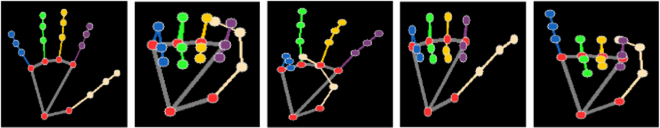
\includegraphics[width=1\linewidth]{gambar/hasilpose.png}
	\caption{Hasil estimasi pose menggunakan \textit{Mediapipe}}
	\label{fig:gambar41}
\end{figure}

\begin{figure}[!h]
	\centering
	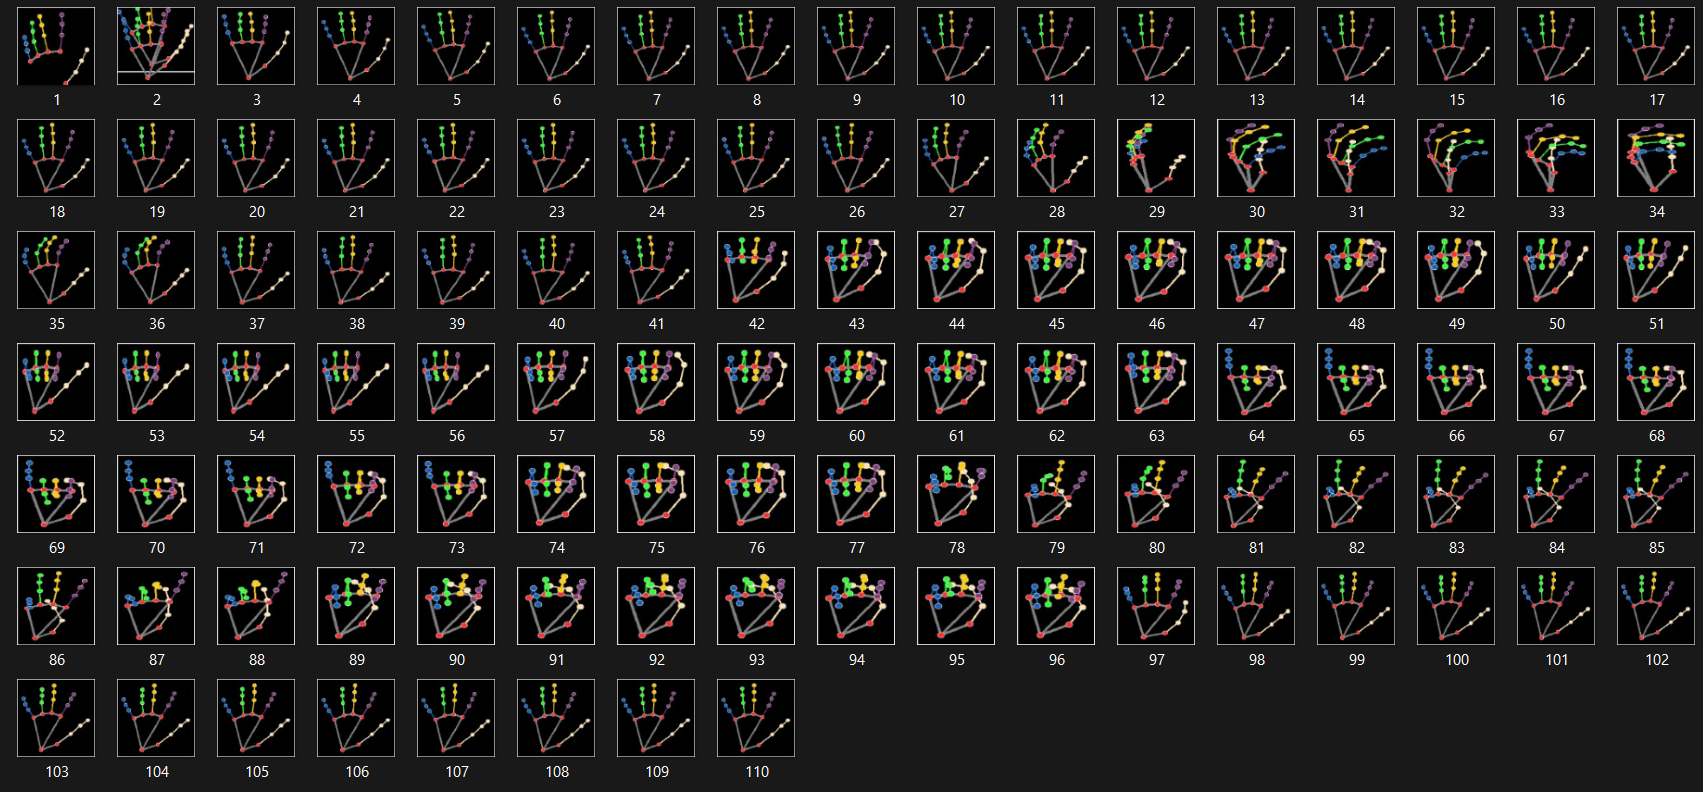
\includegraphics[width=1\linewidth]{gambar/folderdataset.png}
	\caption{Hasil citra yang disimpan}
	\label{fig:gambardatasetfolder}
\end{figure}

